\documentclass[columns=,boxcolor=white]{datart}

%\usepackage[top=1in,bottom=1in,left=1.2in,right=1.2in]{geometry}

%\usepackage{stmaryrd} % For those delicious brackets

% Title
\title{Big Data Problem with Machine Intelligence Stuff}
\date{}

\author[1]{Anders Roland Nielsen}
\author[1]{Andreas Berre Eriksen}
\author[1]{Kent Munthe Caspersen}
\author[1]{Mathias Melgaard Andersen}
\author[1]{Mikkel Alexander Madsen}
\author[1]{Sander Jespersen}

\affil[1]{Department of Computer Science, Aalborg University}

% CLEVEREF
%\crefname{tempDef}{Definition}{Definitions}
%\crefname{tempProof}{Proof}{Proofs}

%COMMANDS

%HÜTTEL RULES
\providecommand{\condinfrule}[3]{\parbox{5.5cm}{\[ {\frac{#1}{#2}}{\qquad #3} \hfill \]}}
\providecommand{\infrule}[2]{\parbox{4.5cm}{\[\frac{#1}{#2}\hspace{.5cm}\]}}
\providecommand{\runa}[1]{\ensuremath{\tt{[#1]}}}
\providecommand{\single}[1]{\ensuremath{#1} \\}
\providecommand{\singlemat}[1]{\parbox{4.5cm}{\[#1\hspace{.5cm}\]}}
\providecommand{\bigrule}[2]{\genfrac{}{}{0pt}{0}{#1}{#2}}

% Gordon
% ----------------------------------------------------------------- %
% Horizontal brackets.                                              %
% ----------------------------------------------------------------- %

\newcommand{\hbra}{
%\hbox to .995       \columnwidth{\vrule width0.3mm height 1.8mm depth-0.3mm
\hbox to .995       \linewidth{\vrule width0.3mm height 1.8mm depth-0.3mm
                    \leaders\hrule height1.8mm depth-1.5mm\hfill
                    \vrule width0.3mm height 1.8mm depth-0.3mm}}
\newcommand{\hket}{
\hbox to .995 
%                    \columnwidth{\vrule width0.3mm height1.5mm
                    \linewidth{\vrule width0.3mm height1.5mm
                    \leaders\hrule height0.3mm\hfill
                    \vrule width0.3mm height1.5mm}}

% ----------------------------------------------------------------- %
% Typesetting definitions:                     output:              %
%                                                                   %
% \begin{defn}                                                      % 
% \Category{M,N}{terms}\\               M, N ::=      terms         %
% \entry{x}{variable}\\                   x             variable    % 
% \entry{M\ N}{application}\\             M N           application %
% \entry{\lambda x.\ M}{abstraction}      \x.M          abstraction %
% \end{defn}                                                        %
%                                                                   %
% This is a tabbing environment; the last entry should have no \\.  %
% ----------------------------------------------------------------- %

\makeatletter
  \newcommand{\addToLabel}[1]{%
    \protected@edef\@currentlabel{\@currentlabel#1}%
  }
\makeatother

\newcommand{\ratio}{.3}

\newenvironment{display}[1]{
  \pagebreak[2]% to prevent ugly broken displays
\begin{tabbing}
%\hspace{1.5em} \= \hspace{\ratio\columnwidth-1.5em} \= \hspace{1.5em} \= \hspace{1.5em} \= \kill
\hspace{1.5em} \= \hspace{\ratio\linewidth-1.5em} \= \hspace{1.5em} \= \hspace{1.5em} \= \kill
  {\bfseries#1}\\[-.7ex]
  \hbra\\[-.6ex]
  }{\\[-.7ex]\hket
  \end{tabbing}\vspace{-1.0ex}\normalsize}

\newcommand{\entry}[2]{\>$#1$\>\>#2}
\newcommand{\clause}[2]{$#1$\>\>#2}
\newcommand{\Category}[2]{\clause{#1::=}{#2}}
\newcommand{\simplecategory}[3]{\clause{#1::=#2}{#3}}
\newcommand{\subclause}[1]{\>\>\>#1}
\newcommand{\redrule}[3]{$#1$\>\>$#2$\>\>\>#3}

\newcommand{\labelledClause}[2]{%
  $#1$
  \>\>\>{\small #2}%
  \refstepcounter{rule}%
  \addToLabel{#2}%
}

\newcommand{\wlabelledClause}[2]{%
  $#1$
  \>\>\>\>{\small #2}%
  \refstepcounter{rule}%
  \addToLabel{#2}%
}


% \newcommand{\nodisplaybreak}[1]{ 
%   \noindent\begin{minipage}{\columnwidth}#1
%   \end{minipage}}

% \newcommand{\nofulldisplaybreak}[1]{ 
%   \iffull\begin{tabbing}\nodisplaybreak{#1}\end{tabbing}\else{#1}\fi}  \hbra\\[-.6ex]
%   }{\\[-.7ex]\hket
%   \end{tabbing}\vspace{-1.0ex}\normalsize}

% \newcommand{\entry}[2]{\>$#1$\>\>#2}
% \newcommand{\clause}[2]{$#1$\>\>#2}
% \newcommand{\Category}[2]{\clause{#1::=}{#2}}
% \newcommand{\simplecategory}[3]{\clause{#1::=#2}{#3}}
% \newcommand{\subclause}[1]{\>\>\>#1}
% \newcommand{\redrule}[3]{$#1$\>\>$#2$\>\>\>#3}




% document
\begin{document}
\maketitle

% ABSTRACT
\begin{abstract}
Here be dragons.
\end{abstract}

%%% Local Variables:
%%% mode: latex
%%% TeX-master: "main"
%%% End:


% CONTENT

\section{Introduction}\label{sec:intro}

Online multiplayer games have the possibility of generating a lot of data, this increases with the possible options for each individual player and the number of players. 
League of Legends (LoL), created by Riot games, was the most played online game in the beginning of 2015~\cite{LoLmostplayed}, mustering 27 million people playing it daily in the beginning of 2014~\cite{LoL27mill}. 

When playing, the players are divided into 2 competing teams (blue, purple) of 5 players each. In a classic match, each player will pick a champion(character) from a pool of 124 champions, each champion with 4 unique abilities. An ability is a magic spell, which does wildly different things, such as throwing a fireball at an opponent.
\\

\begin{wrapfigure}{r}{{0.5\textwidth}}
  \centering
    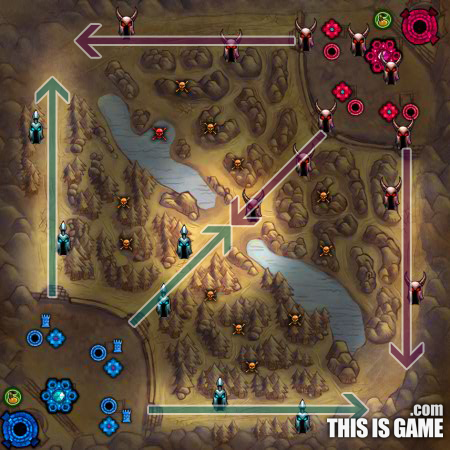
\includegraphics[width=0.5\textwidth]{Section1/lolmap.png}
  \caption{League of legends map}
\end{wrapfigure}\label{lolmap}
The map consists of three lanes(top, middle, bottom) as shown with arrows, connecting the two bases. In front of each lane in each base are two structures, an inhibitor and a turret defending the inhibtor. In the middle of the base is the nexus, which when destroyed ends the game, making the enemy team the winner. In each lane, the inhibitors spawn creeps(small monsters with low damage and health) which walks toward the opposing base on the lane it was spawned, the effect is that the two team's monsters meet in the middle, which is where the teams will fight, killing each others creeps. Furthermore, each lane has two extra turrets outside the base. A turret is a defensive structure fires at approaching enemies. When the inhibitor is destroyed, it makes the opposing team summon stronger minions. Lastly note that there is a "jungle", which consists of stronger monsters which award gold, and experience.
\\
Experience and money is earned through out the game for the individual players, when killing monsters or opposing players. The experience is used to improve the skills of the champion while money is spend purchasing items that will make the player stronger. This sums up the most important aspects of the game, and it is already quite clear how statespace the game hosts. This makes it extremely complex, and very interesting to analyse what one can do to improve ones gameplay. 
\\\\
The game combines strategy, individual player skill, communication and team play. It is a massive skill showcase, but how important is strategy? In this paper we will investigate how much of an advantage one can get by making good strategic decisions, based on a large dataset of matches played.



%\section{Section 2}

%\section{Section 3}



\bibliography{Literature}

% APPENDIX
%\newpage
%\appendix

\end{document}

%%% Local Variables:
%%% mode: latex
%%% TeX-master: t
%%% End:
